\chapter{Introduction}
\pagenumbering{arabic}

Every computer science curriculum in the world includes a course on data
structures and algorithms.  Data structures are \emph{that} important;
they improve our quality of life and even save lives on a regular basis.
Many multi-million and several multi-billion dollar companies have been
built around data structures.

How can this be?  If we stop to think about it, we realize that we
interact with data structures constantly.
\begin{itemize}
  \item  Open a file: File system 
    \index{file system}
    data structures are used to locate
    the parts of that file on disk so they can be retrieved.  This isn't
    easy; disks contain hundreds of millions of blocks.  The contents of your
    file could be stored on any one of them.
  \item Look up a contact on your phone:  A data
    structure is used to lookup a phone number in your contact list
    \index{contact list}
    based on partial
    information even before you finish dialing/typing.  This isn't easy;
    your phone may contain information about a lot of people---everyone
    you have ever contacted via phone or email---and your phone doesn't
    have a very fast processor or a lot of memory.
  \item Log in to your favourite social network:
    \index{social network}
    The network servers
    use your login information to look up your account information.
    This isn't easy; the most popular social networks have hundreds of
    millions of active users.
  \item Do a web search:
    \index{web search}
    The search engine uses data structures to find
    the web pages containing your search terms.  This isn't easy; there
    are over 8.5 billion web pages on the Internet and each page contains
    a lot of potential search terms.
  \item Phone emergency services (9-1-1):
    \index{emergency services}\index{9-1-1}
    The emergency services network
    looks up your phone number in a data structure that maps phone numbers
    to addresses so that police cars, ambulances, or fire trucks can be
    sent there without delay. This is important;  the person making the
    call may not be able to provide the exact address they are calling
    from and a delay can mean the difference between life or death.
\end{itemize}

\section{The Need for Efficiency}

In the next section, we look at the operations supported by the most
commonly used data structures.  Anyone with a bit of programming
experience will see that these operations are not hard to implement
correctly.  We can store the data in an array or a linked list and each
operation can be implemented by iterating over all the elements of the
array or list and possibly adding or removing an element.

This kind of implementation is easy, but not very efficient.  Does this
really matter?  Computers are becoming faster and faster. Maybe the
obvious implementation is good enough. Let's do some rough calculations
to find out.

\paragraph{Number of operations:}  Imagine an application with a
moderately-sized data set, say of one million ($10^6$), items.  It is
reasonable, in most applications, to assume that the application will
want to look up each item at least once.  This means we can expect to do
at least one million ($10^6$) searches in this data.  If each of these
$10^6$ searches inspects  each of the $10^6$ items, this gives a total
of $10^6\times 10^6=10^{12}$ (one thousand billion) inspections.

\paragraph{Processor speeds:} At the time of writing, even a very fast
desktop computer can not do more than one billion ($10^9$) operations per
second.\footnote{Computer speeds are at most a few gigahertz (billions
of cycles per second), and each operation typically takes a few cycles.}
This means that this application will take at least $10^{12}/10^9 = 1000$
seconds, or roughly 16 minutes and 40 seconds.  Sixteen minutes is an
eon in computer time, but a person might be willing to put up with it
(if they were headed out for a coffee break).

%Consider, now an application like the human genome project.  Completed in
%2003 (when computers were quite a bit slower than they are now), this
%was considered an extraordinary scientific accomplishment.  The human
%genome consists of 3 billion ($3\times 10^6$) base pairs. By our
%rough calculations, doing even a single search on this data would take
%3 seconds.  Doing a million searches would take $3$ million seconds,
%or roughly 34 days.  This is starting to get beyond reasonable.

\paragraph{Bigger data sets:} Now consider a company like Google,
\index{Google}
that
indexes over 8.5 billion web pages.  By our calculations, doing any kind
of query over this data would take at least 8.5 seconds.  We already
know that this isn't the case; web searches complete in much less than
8.5 seconds, and they do much more complicated queries than just asking
if a particular page is in their list of indexed pages.  At the time
of writing, Google receives approximately $4,500$ queries per second,
meaning that they would require at least $4,500\times 8.5=38,250$ very
fast servers just to keep up.

\paragraph{The solution:} 
These examples tell us that the obvious implementations of data structures
do not scale well when the number of items, #n#, in the data structure
and the number of operations, $m$, performed on the data structure
are both large.  In these cases, the time (measured in, say, machine
instructions) is roughly $#n#\times m$.

The solution, of course, is to carefully organize data within the data
structure so that not every operation requires every data item to be
inspected.  Although it sounds impossible at first, we will see data
structures where a search requires looking at only two items on average,
independent of the number of items stored in the data structure.  In our
billion instruction per second computer it takes only $0.000000002$
seconds to search in a data structure containing a billion items (or a
trillion, or a quadrillion, or even a quintillion items).

We will also see implementations of data structures that keep the
items in sorted order, where the number of items inspected during an
operation grows very slowly as a function of the number of items in
the data structure.  For example, we can maintain a sorted set of one
billion items while inspecting at most 60 items during any operation.
In our billion instruction per second computer, these operations take
$0.00000006$ seconds each.

The remainder of this chapter briefly reviews some of the main concepts
used throughout the rest of the book.   \secref{interfaces} describes
the interfaces implemented by all of the data structures described in
this book and should be considered required reading.  The remaining
sections discuss:
\begin{itemize}
  \item some mathematical review including exponentials, logarithms,
  factorials, asymptotic (big-Oh) notation, probability, and randomization;
  \item the model of computation; 
  \item correctness, running time, and space;
  \item an overview of the rest of the chapters; and
  \item the sample code and typesetting conventions.
\end{itemize}
A reader with or without a background in these areas can easily skip
them now and come back to them later if necessary.


\section{Interfaces}
\seclabel{interfaces}
When discussing data structures, it is important to understand the
difference between a data structure's interface and its implementation.
An interface describes what a data structure does, while an implementation
describes how the data structure does it.

An \emph{interface},
\index{interface}
\index{abstract data type|see{interface}}
sometimes also called an \emph{abstract data
type}, defines the set of operations supported by a data structure and
the semantics, or meaning, of those operations.  An interface tells us
nothing about how the data structure implements these operations; it only
provides a list of supported operations along with specifications about
what types of arguments each operation accepts and the value returned
by each operation.

A data structure \emph{implementation}, on the other hand, includes the
internal representation of the data structure as well as the definitions
of the algorithms that implement the operations supported by the data
structure.  Thus, there can be many implementations of a single interface.
For example, in \chapref{arrays}, we will see implementations of the
#List# interface using arrays and in \chapref{linkedlists} we will
see implementations of the #List# interface using pointer-based data
structures.  Each implements the same interface, #List#,
but in different ways.

\subsection{The #Queue#, #Stack#, and #Deque# Interfaces}

The #Queue# interface represents a collection of elements to which we
can add elements and remove the next element.  More precisely, the operations
supported by the #Queue# interface are
\begin{itemize}
  \item #add(x)#: add the value #x# to the #Queue#
  \item #remove()#: remove the next (previously added) value, #y#, from the #Queue# and return #y#
\end{itemize}
Notice that the #remove()# operation takes no argument.  The #Queue#'s
\emph{queueing discipline} decides which element should be removed.
There are many possible queueing disciplines, the most common of which
include FIFO, priority, and LIFO.

A \emph{FIFO (first-in-first-out) #Queue#},
\index{FIFO queue}
\index{queue!FIFO}
which is illustrated in
\figref{queue}, removes items in the same order they were added, much
in the same way a queue (or line-up) works when checking out at a cash
register in a grocery store.  This is the most common kind of #Queue#
so the qualifier FIFO is often omitted.  In other texts, the #add(x)#
and #remove()# operations on a FIFO #Queue# are often called #enqueue(x)#
and #dequeue()#, respectively.

\begin{figure}
  \centering{\includegraphics[width=\ScaleIfNeeded]{figs/queue}}
  \caption[A FIFO queue]{A FIFO #Queue#.}
  \figlabel{queue}
\end{figure}

A \emph{priority #Queue#},
\index{priority queue}
\index{priority queue|seealso{heap}}
\index{queue!priority}
illustrated in \figref{prioqueue}, always
removes the smallest element from the #Queue#, breaking ties arbitrarily.
This is similar to the way in which patients are triaged in a hospital
emergency room.  As patients arrive they are evaluated and then placed in
a waiting room.  When a doctor becomes available he or she first treats
the patient with the most life-threatening condition.  The #remove(x)#
operation on a priority #Queue# is usually called #deleteMin()# in
other texts.

\begin{figure}
  \centering{\includegraphics[width=\ScaleIfNeeded]{figs/prioqueue}}
  \caption[A priority queue]{A priority #Queue#.}
  \figlabel{prioqueue}
\end{figure}

%This is similar to the way
%many airlines manage upgrades to the business class on their flights.
%When a business-class seat becomes available it is given to the most
%important customer waiting on an upgrade.

A very common queueing discipline is the LIFO (last-in-first-out)
\index{LIFO queue}
\index{LIFO queue|seealso{stack}}
\index{queue!LIFO}
\index{stack}
discipline, illustrated in \figref{stack}.  In a \emph{LIFO Queue},
the most recently added element is the next one removed.  This is best
visualized in terms of a stack of plates; plates are placed on the top of
the stack and also removed from the top of the stack. This structure is
so common that it gets its own name: #Stack#.  Often, when discussing a
#Stack#, the names of #add(x)# and #remove()# are changed to #push(x)#
and #pop()#; this is to avoid confusing the LIFO and FIFO queueing
disciplines.

\begin{figure}
  \centering{\includegraphics[width=\ScaleIfNeeded]{figs/stack}}
  \caption[A stack]{A stack.}
  \figlabel{stack}
\end{figure}


A #Deque#
\index{deque}
is a generalization of both the FIFO #Queue# and LIFO #Queue#
(#Stack#).   A #Deque# represents a sequence of elements, with a front
and a back.  Elements can be added at the front of the sequence or
the back of the sequence.  The names of the #Deque# operations
are self-explanatory: #addFirst(x)#, #removeFirst()#, #addLast(x)#,
and #removeLast()#.  It is worth noting that a #Stack# can be implemented using only
#addFirst(x)# and #removeFirst()# while a FIFO #Queue# can be implemented
using #addLast(x)# and #removeFirst()#.


\subsection{The #List# Interface: Linear Sequences}

This book will talk very little about the FIFO #Queue#, #Stack#, or
#Deque# interfaces.  This is because these interfaces are subsumed by the
#List# interface.  A #List#,
\index{List@#List#}
illustrated in \figref{list}, represents a
sequence, $#x#_0,\ldots,#x#_{#n#-1}$, of values.  The #List# interface
includes the following operations:

\begin{enumerate}
  \item #size()#: return #n#, the length of the list
  \item #get(i)#: return the value $#x#_{#i#}$
  \item #set(i,x)#: set the value of $#x#_{#i#}$ equal to #x#
  \item #add(i,x)#: add #x# at position #i#, displacing
    $#x#_{#i#},\ldots,#x#_{#n#-1}$; \\ 
    Set $#x#_{j+1}=#x#_j$, for all
    $j\in\{#n#-1,\ldots,#i#\}$, increment #n#, and set $#x#_i=#x#$
  \item #remove(i)# remove the value $#x#_{#i#}$, displacing
    $#x#_{#i+1#},\ldots,#x#_{#n#-1}$; \\ 
    Set $#x#_{j}=#x#_{j+1}$, for all
    $j\in\{#i#,\ldots,#n#-2\}$ and decrement #n#
\end{enumerate}
Notice that these operations are easily sufficient to implement the
#Deque# interface:
\begin{eqnarray*}
  #addFirst(x)# &\Rightarrow& #add(0,x)# \\
  #removeFirst()# &\Rightarrow& #remove(0)#  \\
  #addLast(x)# &\Rightarrow& #add(size(),x)# \\
  #removeLast()# &\Rightarrow& #remove(size()-1)#
\end{eqnarray*}

\begin{figure}
  \centering{\includegraphics[width=\ScaleIfNeeded]{figs/list}}
  \caption[A List]{A #List# represents a sequence indexed by
   $0,1,2,\ldots,#n#$.  In this #List# a call to #get(2)# would return
   the value $c$.}
  \figlabel{list}
\end{figure}

Although we will normally not discuss the #Stack#, #Deque# and FIFO
#Queue# interfaces in subsequent chapters, the terms #Stack# and #Deque#
are sometimes used in the names of data structures that implement the
#List# interface.  When this happens, it highlights the fact that
these data structures can be used to implement the #Stack# or #Deque#
interface very efficiently.  For example, the #ArrayDeque# class is an
implementation of the #List# interface that implements all the #Deque#
operations in constant time per operation.


\subsection{The #USet# Interface: Unordered Sets}

The #USet#
\index{USet@#USet#}
interface represents an unordered set of unique elements, which
mimics a mathematical \emph{set}. A #USet# contains #n# \emph{distinct}
elements; no element appears more than once; the elements are in no
specific order.  A #USet# supports the following operations:

\begin{enumerate}
  \item #size()#: return the number, #n#, of elements in the set
  \item #add(x)#: add the element #x# to the set if not already present; \\
    Add #x# to the set provided that there
    is no element #y# in the set such that #x# equals #y#.  Return #true#
    if #x# was added to the set and #false# otherwise.
  \item #remove(x)#: remove #x# from the set; \\
    Find an element #y# in the set such that #x# equals
    #y# and remove #y#.  Return #y#, or #null# if no such element exists.
  \item #find(x)#: find #x# in the set if it exists; \\
    Find an element #y# in the set such that #y# equals
    #x#.  Return #y#, or #null# if no such element exists.
\end{enumerate}

These definitions are a bit fussy about distinguishing #x#, the element
we are removing or finding, from #y#, the element we may remove or find.
This is because #x# and #y# might actually be distinct objects that
are nevertheless treated as equal.\javaonly{\footnote{In Java, this is
done by overriding the class's #equals(y)# and #hashCode()# methods.}}
Such a distinction is  useful because it allows for the creation of
\emph{dictionaries} or \emph{maps} that map keys onto values.
\index{dictionary}
\index{map}

To create a dictionary/map, one forms compound objects called #Pair#s,
\index{pair}
each of which contains a \emph{key} and a \emph{value}. Two #Pair#s
are treated as equal if their keys are equal.  If we store some pair
$(#k#,#v#)$ in a #USet# and then later call the #find(x)# method using
the pair $#x#=(#k#,#null#)$ the result will be $#y#=(#k#,#v#)$.  In other
words, it is possible to recover the value, #v#, given only the key, #k#.


\subsection{The #SSet# Interface: Sorted Sets}
\seclabel{sset}

\index{SSet@#SSet#}
The #SSet# interface represents a sorted set of elements.  An #SSet#
stores elements from some total order, so that any two elements #x#
and #y# can be compared.  In code examples, this will be done with a
method called #compare(x,y)# in which
\[
    #compare(x,y)# 
      \begin{cases}
        {}<0 & \text{if $#x#<#y#$} \\
        {}>0 & \text{if $#x#>#y#$} \\
        {}=0 & \text{if $#x#=#y#$}
      \end{cases}
\]
\index{compare@#compare(x,y)#}
An #SSet# supports the #size()#, #add(x)#, and #remove(x)# methods with
exactly the same semantics as in the #USet# interface.  The difference
between a #USet# and an #SSet# is in the #find(x)# method:
\begin{enumerate}
\setcounter{enumi}{3}
\item #find(x)#: locate #x# in the sorted set; \\
   Find the smallest element #y# in the set such that $#y# \ge #x#$.
   Return #y# or #null# if no such element exists.
\end{enumerate}

This version of the #find(x)# operation is sometimes referred to
as a \emph{successor search}.
\index{successor search}
It differs in a fundamental way from
#USet.find(x)# since it returns a meaningful result even when there is
no element equal to #x# in the set.

The distinction between the #USet# and #SSet# #find(x)# operations is
very important and is often missed.  The extra functionality provided
by an #SSet# usually comes with a price that includes both a larger
running time and a higher implementation complexity.  For example, most
of the #SSet# implementations discussed in this book all have #find(x)#
operations with running times that are logarithmic in the size of the set.
On the other hand, the implementation of a #USet# as a #ChainedHashTable#
in \chapref{hashing} has a #find(x)# operation that runs in constant
expected time.  When choosing which of these structures to use, one should
always use a #USet# unless the extra functionality offered by an #SSet#
is truly needed.

% \subsection{The DynamicString Interface}

\section{Mathematical Background}

In this section, we review some mathematical notations and tools
used throughout this book, including logarithms, big-Oh notation, and
probability theory.  This review will be brief and is not intended as
an introduction. Readers who feel they are missing this background are
encouraged to read, and do exercises from, the appropriate sections of
the very good (and free) textbook on mathematics for computer science
\cite{llm11}.

\subsection{Exponentials and Logarithms}

\index{exponential}
The expression $b^x$ denotes the number $b$ raised to the power of $x$.
If $x$ is a positive integer, then this is just the value of $b$
multiplied by itself $x-1$ times:
\[
    b^x = \underbrace{b\times b\times \cdots \times b}_{x} \enspace .
\]
When $x$ is a negative integer, $b^x=1/b^{-x}$.  When $x=0$, $b^x=1$.
When $b$ is not an integer, we can still define exponentiation in terms
of the exponential function $e^x$ (see below), which is itself defined in
terms of the exponential series, but this is best left to a calculus text.

\index{logarithm}
In this book, the expression $\log_b k$ denotes the \emph{base-$b$ logarithm}
of $k$.  That is, the unique value $x$ that satisfies
\[
    b^{x} = k  \enspace .
\]
Most of the logarithms in this book are base 2 (\emph{binary logarithms}),
\index{binary logarithm}
\index{logarithm!binary} 
in which case we drop the base, so that $\log k$ is shorthand for
$\log_2 k$.

An informal, but useful, way to think about logarithms is to think
of $\log_b k$ as the number of times we have to divide $k$ by $b$
before the result is less than or equal to 1.  For example, when one
does binary search, each comparison reduces the number of possible
answers by a factor of 2.  This is repeated until there is at most one
possible answer.  Therefore, the number of comparison done by binary
search when there are initially at most $n+1$ possible answers is at
most $\lceil\log_2(n+1)\rceil$.

\index{natural logarithm}
\index{logarithm!natural} 
Another logarithm that comes up several times in this book is the
\emph{natural logarithm}.  Here we use the notation $\ln k$ to denote
$\log_e k$, where $e$ --- \emph{Euler's constant} --- is given by
\index{Euler's constant}
\index{e@$e$}
\[
   e = \lim_{n\rightarrow\infty} \left(1+\frac{1}{n}\right)^n
   \approx  2.71828 \enspace .
\]
The natural logarithm comes up frequently because it is the value
of a particularly common integral:
\[
    \int_{1}^{k} 1/x\,\mathrm{d}x  = \ln k \enspace .
\]
Two of the most common manipulations we do with logarithms are removing
them from an exponent:
\[
    b^{\log_b k} = k
\]
and changing the base of a logarithm:
\[
    \log_b k = \frac{\log_a k}{\log_a b} \enspace .
\]
For example, we can use these two manipulations to compare the natural and binary logarithms
\[
   \ln k = \frac{\log k}{\log e} = \frac{\log k}{(\ln e)/(\ln 2)} = 
    (\ln 2)(\log k) \approx 0.693147\log k \enspace .
\]

\subsection{Factorials}
\seclabel{factorials}

\index{factorial}
In one or two places in this book, the \emph{factorial} function is used.
For a non-negative integer $n$, the notation $n!$ (pronounced ``$n$ factorial'') is defined to mean 
\[
   n! = 1\cdot2\cdot3\cdot\cdots\cdot n \enspace .
\]
Factorials appear because $n!$ counts the number of distinct
permutations, i.e., orderings, of $n$ distinct elements.
\index{permutation}
For the special case $n=0$, $0!$ is defined as 1. 

\index{Stirling's Approximation}
The quantity $n!$ can be approximated using \emph{Stirling's Approximation}:
\[
	n! 
   = \sqrt{2\pi n}\left(\frac{n}{e}\right)^{n}e^{\alpha(n)} \enspace ,
\]
where
\[  
   \frac{1}{12n+1} <  \alpha(n) < \frac{1}{12n}  \enspace .
\]
Stirling's Approximation also approximates $\ln(n!)$:
\[
   \ln(n!) = n\ln n - n + \frac{1}{2}\ln(2\pi n) + \alpha(n)
\]
(In fact, Stirling's Approximation is most easily proven by approximating
$\ln(n!)=\ln 1 + \ln 2  + \cdots + \ln n$ by the integral
$\int_1^n \ln n\,\mathrm{d}n = n\ln n - n +1$.)

\index{binomial coefficients}
Related to the factorial function are the \emph{binomial coefficients}.
For a non-negative integer $n$ and an integer $k\in\{0,\ldots,n\}$,
the notation $\binom{n}{k}$ denotes:
\[
   \binom{n}{k} = \frac{n!}{k!(n-k)!} \enspace .
\]
The binomial coefficient $\binom{n}{k}$ (pronounced ``$n$ choose $k$'')
counts the number of subsets of an $n$ element set that have size $k$,
i.e., the number of ways of choosing $k$ distinct integers from the
set $\{1,\ldots,n\}$.

\subsection{Asymptotic Notation}

\index{asymptotic notation}
\index{big-Oh notation}
\index{O@$O$ notation}
When analyzing data structures in this book, we want to talk about
the running times of various operations.  The exact running times will,
of course, vary from computer to computer and even from run to run on an
individual computer.  When we talk about the running time of an operation
we are referring to the number of computer instructions performed during
the operation.  Even for simple code, this quantity can be difficult to
compute exactly.  Therefore, instead of analyzing running times exactly,
we will use the so-called \emph{big-Oh notation}: For a function $f(n)$,
$O(f(n))$ denotes a set of functions,
\[
   O(f(n)) = \left\{
     \begin{array}{l}
       g(n):\mbox{there exists $c>0$, and $n_0$ such that} \\
             \quad\mbox{$g(n) \le c\cdot f(n)$ for all $n\ge n_0$}   
     \end{array} \right\} \enspace .
\]
Thinking graphically, this set consists of the functions $g(n)$ where
$c\cdot f(n)$ starts to dominate $g(n)$ when $n$ is sufficiently large.

We generally use asymptotic notation to simplify functions.  For example,
in place of $5n\log n + 8n - 200$ we can write $O(n\log n)$.
This is proven as follows:
\begin{align*} 
       5n\log n + 8n - 200
        & \le 5n\log n + 8n \\
        & \le 5n\log n + 8n\log n & \mbox{ for $n\ge 2$ (so that $\log n \ge 1$)}
            \\
        & \le 13n\log n  \enspace .
\end{align*}
This demonstrates that the function $f(n)=5n\log n + 8n - 200$ is in
the set $O(n\log n)$ using the constants $c=13$ and $n_0 = 2$.

A number of useful shortcuts can be applied when using asymptotic
notation.  First:
\[ O(n^{c_1}) \subset O(n^{c_2}) \enspace ,\]
for any $c_1 < c_2$.  Second: For any constants $a,b,c > 0$,
\[ O(a) \subset O(\log n) \subset O(n^{b}) \subset O({c}^n) \enspace . \]
These inclusion relations can be multiplied by any positive value,
and they still hold. For example, multiplying by $n$ yields:
\[ O(n) \subset O(n\log n) \subset O(n^{1+b}) \subset O(n{c}^n) \enspace . \]

Continuing in a long and distinguished tradition, we will abuse this
notation by writing things like $f_1(n) = O(f(n))$ when what we really
mean is $f_1(n) \in O(f(n))$.  We will also make statements like ``the
running time of this operation is $O(f(n))$'' when this statement should
be ``the running time of this operation is \emph{a member of} $O(f(n))$.''
These shortcuts are mainly to avoid awkward language and to make it
easier to use asymptotic notation within strings of equations.

A particularly strange example of this occurs when we write statements like
\[
  T(n) = 2\log n + O(1)  \enspace .
\]
Again, this would be more correctly written as
\[
  T(n) \le 2\log n + [\mbox{some member of $O(1)$]}  \enspace .
\]

The expression $O(1)$ also brings up another issue. Since there is
no variable in this expression, it may not be clear which variable is
getting arbitrarily large.  Without context, there is no way to tell.
In the example above, since the only variable in the rest of the equation
is $n$, we can assume that this should be read as $T(n) = 2\log n +
O(f(n))$, where $f(n) = 1$.

Big-Oh notation is not new or unique to computer science.  It was
used by the number theorist Paul Bachmann as early as 1894, and is
immensely useful for describing the running times of computer algorithms.
Consider the following piece of code:
\javaimport{junk/Simple.snippet()}
\cppimport{ods/Simple.snippet()}
One execution of this method involves
\begin{itemize}
      \item $1$ assignment (#int\, i\, =\, 0#),
      \item $#n#+1$ comparisons (#i < n#),
      \item #n# increments (#i++#),
      \item #n# array offset calculations (#a[i]#), and
      \item #n# indirect assignments (#a[i] = i#).
\end{itemize}
So we could write this running time as
\[
    T(#n#)=a + b(#n#+1) + c#n# + d#n# + e#n# \enspace , 
\]
where $a$, $b$, $c$, $d$, and $e$ are constants that depend on the
machine running the code and represent the time to perform assignments,
comparisons, increment operations, array offset calculations, and indirect
assignments, respectively.  However, if this expression represents the
running time of two lines of code, then clearly this kind of analysis
will not be tractable to complicated code or algorithms.  Using big-Oh
notation, the running time can be simplified to
\[
    T(#n#)= O(#n#) \enspace .
\]
Not only is this more compact, but it also gives nearly as much
information.  The fact that the running time depends on the constants $a$,
$b$, $c$, $d$, and $e$ in the above example means that, in general, it
will not be possible to compare two running times to know which is faster
without knowing the values of these constants.  Even if we make the
effort to determine these constants (say, through timing tests), then
our conclusion will only be valid for the machine we run our tests on.

Big-Oh notation allows us to reason at a much higher level, making
it possible to analyze more complicated functions.  If two algorithms
have the same big-Oh running time, then we won't know which is faster,
and there may not be a clear winner.  One may be faster on one machine,
and the other may be faster on a different machine.  However, if the
two algorithms have demonstrably different big-Oh running times, then
we can be certain that the one with the smaller running time will be
faster \emph{for large enough values of #n#}.

An example of how big-Oh notation allows us to compare two different
functions is shown in \figref{intro-asymptotics}, which compares the rate
of grown of $f_1(#n#)=15#n#$ versus $f_2(n)=2#n#\log#n#$.  It might be
that $f_1(n)$  is the running time of a complicated linear time algorithm
while $f_2(n)$ is the running time of a considerably simpler algorithm
based on the divide-and-conquer paradigm.  This illustrates that,
although $f_1(#n#)$ is greater than $f_2(n)$ for small values of #n#,
the opposite is true for large values of #n#.  Eventually $f_1(#n#)$
wins out, by an increasingly wide margin.  Analysis using big-Oh notation
told us that this would happen, since $O(#n#)\subset O(#n#\log #n#)$.

\begin{figure}
  \begin{center}
    \documentclass[xcolor=dvipsnames]{beamer}
\usepackage{comp2402}
\title{Big O: A Review}
\author{Pat Morin \\ COMP2402/2002}
\date{Carleton University}

\begin{document}

\begin{frame}
  \titlepage
\end{frame}

\begin{frame}
  \frametitle{Big O: Definition} 
   \[ \begin{array}{ll} O(g(n)) = \{ f(n) : &
          \mbox{there exists positive constants $c$ and $n_0$} \\
          & \mbox{such that $f(n) \le cg(n)$ for all $n\ge n_0$} \}\end{array} 
   \]
  \begin{itemize}
  \item<2-> Notice: $O(g(n))$ is a set of functions
   \begin{itemize}
     \item<3-> When we say $f(n)=O(g(n))$ we really mean $f(n)\in O(g(n))$
     \item<4-> E.g., $n^2 + 42n + 7 = O(n^2)$ means:
     \begin{itemize}
       \item<4-> The function $f(n)=n^2 + 42n + 7$ is in the set $O(n^2)$
     \end{itemize}
   \end{itemize}
  \end{itemize}

\end{frame}

\begin{frame}
  \frametitle{$n^2 + 42n + 7 = O(n^2)$}
  \begin{center}
    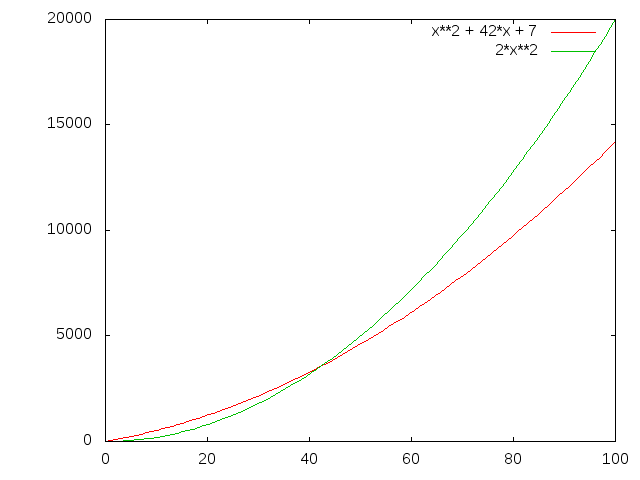
\includegraphics[height=2.5in]{images/graph} \\
    $n^2 + 42n + 7 \le 2 n^2$ for all $n\ge 50$
  \end{center}
\end{frame}

\begin{frame}
  \frametitle{Example}

  \begin{itemize}
    \item Prove $n^2 + 42n + 7 = O(n^2)$
    \item<2-> \[\begin{aligned} 
       n^2 + 42n + 7 
        & \le n^2 + 42n^2 + 7n^2 & \mbox{ for $n\ge 1$} \\ 
        & = 50n^2
      \end{aligned}\]
    \item<3-> So, $n^2 + 42n + 7 \le 50 n^2$ for all $n\ge 1$
    \item<4-> $n^2 + 42n^2 + 7n^2 = O(n^2)$  [ $c=50$, $n_0=1$ ]
  \end{itemize}
\end{frame}

\begin{frame}
  \frametitle{Example}

  \begin{itemize}
    \item Prove $5n\log_2 n + 8n - 200 = O(n\log_2 n)$
    \item<2->[] \[\begin{aligned} 
       5n\log_2 n + 8n - 200
        & \le 5n\log_2 n + 8n \\
        & \le 5n\log_2 n + 8n\log_2 n & \mbox{ for $n\ge 2$ ($\log_2 n \ge 1$)}
            \\
        & \le 13n\log_2 n 
      \end{aligned}\]
    \item<3-> $5n\log_2 n + 8n - 200 \le 13n\log_2 n$ for all $n\ge 2$
    \item<4-> $5n\log_2 n + 8n - 200 = O(n\log_2 n)$ [ $c=13$, $n_0=2$ ]
  \end{itemize}
\end{frame}

\begin{frame}
  \frametitle{Some common relations}

  \begin{itemize}
    \item $O(n^{c_1}) \subset O(n^{c_2})$ for any $c_1 < c_2$
    \item For any constants $a,b,c > 0$,
     \[ O(a) \subset O(\log n) \subset O(n^{b}) \subset O({c}^n) \]
    \item<2-> These make things faster
     \[ 2\log_2 n + 2 = O(\log n) \]
     \[ n + 2 = O(n) \]
     \[ 2n + 15n^{1/2} = O(n) \]
   \item<3-> We can multiply these to learn about other functions,
     \[ O(an) = O(n) \subset O(n\log n) \subset O(n^{1+b}) \subset O(n{c}^n) \]
   \item<4->Examples: $O(n^{1.5}) \subseteq O(n^{1.5}\log n)$
  \end{itemize}
\end{frame}

\begin{frame}
  \frametitle{An indulgence}

  \begin{itemize}
    \item In this course, we see expressions like $O(n-i)$
    \begin{itemize}
      \item Two argument function $g(n,i)=n-i$
      \item \emph{For the purposes of this course}, 
               we will take $O(g(n,i))$ to be
       \[ \begin{array}{ll} O(g(n,i)) = \{ f(n,i) : &
           \mbox{there exists positive constants $c$ and $z$} \\
           & \mbox{such that $f(n,i) \le cg(n,i)$ for all } \\
           & \mbox{arguments such that $f(n,i)>z$} \}\end{array} 
       \]
    \end{itemize}
    \item For example (Lists) valid arguments are $i\in\{0,\ldots,n-1\}$ or (sometimes) $i\in\{0,\ldots,n\}$
  \end{itemize}
\end{frame}

\begin{frame}[fragile]
  \frametitle{Why Use big-O Notation?}
   
  \begin{itemize}
    \item Consider the following (simple) code:
\begin{lstlisting}
  for (int i = 0; i < n; i++) {
    a[i] = i;
  } 
\end{lstlisting}
   \item<2-> The running time is 
   \begin{itemize}
      \item<3-> 1 assignment (\lstinline{int i = 0})
      \item<4-> n+1 comparisons (\lstinline{i < n})
      \item<5-> n increments (\lstinline{i++})
      \item<6-> n array offset calculations (\lstinline{a[i]})
      \item<7-> n indirect assignments (\lstinline{a[i] = i})
      \item<8-> ${}=a + b(n+1) + cn + dn + en$, where $a$, $b$, $c$, $d$, and $e$ are constants that depend on the machine running the code

   \end{itemize}
   \item<9-> Easier just to say $O(n)$ (constant-time) operations
 \end{itemize}

\end{frame}
\end{document}




%\section[Outline]{}
%\frame{\tableofcontents}
%

\section{Convex Hulls}
\frame
{
  \frametitle{Convex Hulls}
  
  \begin{itemize}
    \item Let $P=\{p_0,\ldots,p_{n-1}\}$ be a set of points in the plane
    \item The \emph{convex hull} of $S$
     \begin{itemize}
       \item the smallest convex set that contains $S$.
       \item<2->stretch a rubber band around $S$\only<3->{ and let it go}
    \end{itemize}
    \begin{center}
      \only<1>{\includegraphics{figs/ch-a}} %
      \only<2>{\includegraphics{figs/ch-b}} %
      \only<3->{\includegraphics{figs/ch-c}} %
    \end{center}
  \end{itemize}
}

\frame
{
  \frametitle{Upper and Lower Hulls}
  \begin{itemize}
    \item The \emph{upper hull} of $S$ is a bit simpler
    \begin{itemize}
      \item<2-> get a rope with weights on both ends \only<3->{and throw it over $S$}
    \end{itemize}
    \item<4->For the \emph{lower hull}, use helium-baloons
    \item<5->Convex hull = upper hull + lower hull
  \end{itemize}
    \begin{center}
      \only<1>{\includegraphics{figs/ch-a}} %
      \only<2>{\includegraphics{figs/ch-d}} %
      \only<3>{\includegraphics{figs/ch-e}} %
      \only<4>{\includegraphics{figs/ch-f}} %
      \only<5->{\includegraphics{figs/ch-g}} %
    \end{center}
}

\frame
{
  \frametitle{Summary so far}
  \begin{itemize}
  \item<1-> Input: A set $P$ of $n$ points (unordered)
  \item<2-> Output: A list of the points of $P$ on the convex hull --- in clockwise order
  \item<3-> First compute the upper hull, then the lower hull
  \end{itemize}
  \begin{center}
    \only<1>{\includegraphics{figs/ch-io-a}}%
    \only<2->{\includegraphics{figs/ch-io-b}}%
  \end{center}
}

\frame
{
  \frametitle{Graham's Scan}

  \begin{tabular}{p{3in}p{1.5in}}
    {\vspace{-2in} \begin{itemize}
      \item<1->Invented by Ron Graham in 1973
      \item<2->Sorts the points by $x$-coordinate
      \item<3->Constructs the upper hull incrementally using a stack
    \end{itemize} }
    &
    {\includegraphics[height=2in]{images/graham-12ball} }
  \end{tabular}
}

\frame{
  \frametitle{Graham's Scan}

  \begin{enumerate}
  \item<2->Sort the points by $x$-coordinate
  \item<3->Create a stack $s$ containing $\langle p_0,p_1\rangle$
  \item<4->For $i=3$ to $n$ do
   \begin{itemize}
    \item add $p_i$ to the convex hull of $p_1,\ldots,p_{i-1}$
   \end{itemize}
  \end{enumerate}
  \begin{center}
    \only<1>{\includegraphics{figs/ch-graham-a}}%
    \only<2>{\includegraphics{figs/ch-graham-b}}%
    \only<3>{\includegraphics{figs/ch-graham-c}}%
    \only<4>{\includegraphics{figs/ch-graham-d}}%
    \only<5>{\includegraphics{figs/ch-graham-e}}%
    \only<6>{\includegraphics{figs/ch-graham-f}}%
    \only<7>{\includegraphics{figs/ch-graham-g}}%
    \only<8>{\includegraphics{figs/ch-graham-h}}%
    \only<9>{\includegraphics{figs/ch-graham-i}}%
    \only<10>{\includegraphics{figs/ch-graham-j}}%
    \only<11>{\includegraphics{figs/ch-graham-k}}%
    \only<12>{\includegraphics{figs/ch-graham-l}}%
    \only<13>{\includegraphics{figs/ch-graham-m}}%
    \only<14->{\includegraphics{figs/ch-graham-n}}%
  \end{center}
}

\frame
{
  \frametitle{Adding $p_i$}
  \begin{itemize}
    \item Suppose #s# contains the upper hull of $p_0,\ldots,p_{i-1}$
    \item We want to compute upper hull of $p_0,\ldots,p_{i}$
    \begin{enumerate}
    \item while #s.get(s.size()-2)#, #s.get(s.size()-1)#, and $p_i$ form a left turn
    \begin{itemize}
      \item #s.remove(s.size()-1)# (pop)
    \end{itemize}
    \item  #s.add(#$p_i$#)#
    \end{enumerate}
  \end{itemize}
  \begin{center}
    \only<1>{\includegraphics{figs/ch-graham-e}}%
    \only<2>{\includegraphics{figs/ch-graham-e-a}}%
    \only<3>{\includegraphics{figs/ch-graham-e-b}}%
    \only<4>{\includegraphics{figs/ch-graham-e-c}}%
    \only<5>{\includegraphics{figs/ch-graham-e-d}}%
    \only<6>{\includegraphics{figs/ch-graham-e-d}}%
  \end{center}
}


\begin{frame}[fragile]
  \frametitle{Graham's Scan -- in Java}

\begin{code}
  public static List<Point2D>
       grahamScan(List<Point2D> p) {
    Collections.sort(p, new XComparator());
    List<Point2D> s = new ArrayList<Point2D>();
    s.add(p.get(0)); s.add(p.get(1));
    for (int i = 2; i < p.size(); i++) {
      Point2D pi = p.get(i);
      while (s.size() >= 2 
          && leftTurn(s.get(s.size()-2), 
                      s.get(s.size()-1), 
                      pi)) {
        s.remove(s.size());    // pop
      }
      s.add(pi);
    }
    return s;
  }
\end{code}
\end{frame}

\begin{frame}
  \frametitle{Analysis of Graham's Scan}

  \begin{itemize}
    \item<1-> Graham's Scan first sorts the data
    \begin{itemize}
      \item can be done $O(n\log n)$ time (see COMP3804)
    \end{itemize}
    \item<2-> Creates a stack and pushes two values
    \begin{itemize}
      \item takes $O(1)$ time
    \end{itemize}
    \item<3-> A #for# loop over $n-2=O(n)$ values
    \begin{itemize}
      \item<4-> each iteration does some #pop#/#remove# operations
       \begin{itemize}
        \item how many?
      \end{itemize}
      \item<5-> each iteration does 1 #push#/#add# operation
      \begin{itemize}
        \item $O(1)$ per iteration = $O(n)$ overall
      \end{itemize}
    \end{itemize}
    \item<6->Total: $O(n\log n) + O(n)$
         \only<6>{${} + O(\mbox{num. #pop# operations})$}
         \only<7->{${} + O(n)$}
         \only<8->{${} =  O(n\log n) $}
  \end{itemize}
\end{frame}

\begin{frame}
  \frametitle{Summary}

  \begin{itemize}
    \item<1-> \textbf{Theorem:} Given a collection $P$ of $n$ points in the plane, Graham's Scan can compute their upper hull in $O(n\log n)$ time.
    \item<2-> With two passes, we can compute the upper hull and lower hull and attach them together to get the convex hull:
    \item<3-> \textbf{Theorem:} Given a collection $P$ of $n$ points in the plane, two applications of Graham's Scan can compute their convex hull in $O(n\log n)$ time.
    \item<4-> By using a Deque, we only need one pass
  \end{itemize}
\end{frame}


\begin{frame}
  \frametitle{Graham's Scan with a deque}
  \begin{itemize}
    \item<1-> Graham's Scan can compute the convex hull in one-pass using a deque
    \begin{center}
      \only<1>{\includegraphics{figs/ch-graham-deque-a}}%
      \only<2>{\includegraphics{figs/ch-graham-deque-b}}%
      \only<3>{\includegraphics{figs/ch-graham-deque-c}}%
      \only<4>{\includegraphics{figs/ch-graham-deque-d}}%
      \only<5>{\includegraphics{figs/ch-graham-deque-e}}%
      \only<6>{\includegraphics{figs/ch-graham-deque-f}}%
      \only<7>{\includegraphics{figs/ch-graham-deque-g}}%
    \end{center}
  \end{itemize}
\end{frame}

\begin{frame}
  \frametitle{Melkman's Algorithm}

  \begin{tabular}{p{3in}p{1.5in}}
  \vspace{-1.5in}\begin{itemize}
    \item<1-> Graham's Scan starts by sorting the the points by $x$-coordinate
    \begin{itemize}
     \item<2->This means that $p_0,\ldots,p_{n-1}$ becomes a non-self-intersecting path
     \item<2->If points are already sorted then Graham's Scan takes $O(n)$ time
    \end{itemize}
    \item<3-> Melkman's Algorithm:
    \begin{itemize}
      \item<4->Works for any non-self-intersecting path $p_0,\ldots,p_{n-1}$
    \end{itemize}
  \end{itemize}
  \begin{center}
    \only<1>{\includegraphics[height=1.2in]{figs/ch-melkman-a}}
    \only<2-3>{\includegraphics[height=1.2in]{figs/ch-melkman-b}}
    \only<4->{\includegraphics[height=1.2in]{figs/ch-melkman-c}}
  \end{center}
  & 
  \includegraphics[height=1.5in]{images/melkman}
  \end{tabular}
\end{frame}




\end{document}


  \end{center}
  \caption{Plots of $15#n#$ versus $2#n#\log#n#$.}
  \figlabel{intro-asymptotics}
\end{figure}

In a few cases, we will use asymptotic notation on functions with more
than one variable. There seems to be no standard for this, but for our
purposes, the following definition is sufficient:
\[
   O(f(n_1,\ldots,n_k)) = 
   \left\{\begin{array}{@{}l@{}}
             g(n_1,\ldots,n_k):\mbox{there exists $c>0$, and $z$ such that} \\
             \quad \mbox{$g(n_1,\ldots,n_k) \le c\cdot f(n_1,\ldots,n_k)$} \\
             \qquad \mbox{for all $n_1,\ldots,n_k$ such that $g(n_1,\ldots,n_k)\ge z$}   
   \end{array}\right\} \enspace .
\]
This definition captures the situation we really care about:  when the
arguments $n_1,\ldots,n_k$ make $g$ take on large values.  This definition
also agrees with the univariate definition of $O(f(n))$ when $f(n)$
is an increasing function of $n$.  The reader should be warned that,
although this works for our purposes, other texts may treat multivariate
functions and asymptotic notation differently.


\subsection{Randomization and Probability}
\seclabel{randomization}

\index{randomization}
\index{probability}
\index{randomized data structure}
\index{randomized algorithm}
Some of the data structures presented in this book are \emph{randomized};
they make random choices that are independent of the data being stored
in them or the operations being performed on them.  For this reason,
performing the same set of operations more than once using these
structures could result in different running times.  When analyzing these
data structures we are interested in their average or \emph{expected}
running times.
\index{expected running time}
\index{running time!expected}

Formally, the running time of an operation on a randomized data structure
is a random variable, and we want to study its \emph{expected value}.
\index{expected value}
For
a discrete random variable $X$ taking on values in some countable
universe $U$, the expected value of $X$, denoted by $\E[X]$, is given
by the formula
\[
    \E[X] = \sum_{x\in U} x\cdot\Pr\{X=x\} \enspace .
\]
Here $\Pr\{\mathcal{E}\}$ denotes the probability that the event
$\mathcal{E}$ occurs.  In all of the examples in this book, these
probabilities are only with respect to the random choices made by the
randomized data structure;  there is no assumption that the data stored
in the structure nor that the sequence of operations performed on the
data structure is random.

One of the most important properties of expected values is \emph{linearity
of expectation}.
\index{linearity of expectation}
For any two random variables $X$ and $Y$,
\[
   \E[X+Y] = \E[X] + \E[Y] \enspace .
\]
More generally, for any random variables $X_1,\ldots,X_k$,
\[
   \E\left[\sum_{i=1}^k X_k\right] = \sum_{i=1}^k \E[X_i] \enspace .
\]
Linearity of expectation allows us to break down complicated random variables (like the left hand sides of the above equations) into sums of simpler random variables (the right hand sides).

A useful trick, that we will use repeatedly, is defining \emph{indicator
random variables}.
\index{indicator random variable}
These binary variables are useful when we want to
count something and are best illustrated by an example.  Suppose we toss
a fair coin $k$ times and we want to know the expected number of times
the coin turns up as heads.
\index{coin toss}
Intuitively, we know the answer is $k/2$,
but if we try to prove it using the definition of expected value, we get
\begin{align*}
   \E[X] & = \sum_{i=0}^k i\cdot\Pr\{X=i\} \\
         & = \sum_{i=0}^k i\cdot\binom{k}{i}/2^k \\
         & = k\cdot \sum_{i=0}^{k-1}\binom{k-1}{i}/2^k \\
         & = k/2 \enspace .
\end{align*}
This requires that we know enough to calculate that $\Pr\{X=i\}
= \binom{k}{i}/2^k$, and that we know the binomial identities
$i\binom{k}{i}=k\binom{k-1}{i}$ and $\sum_{i=0}^{k} \binom{k}{i} = 2^{k}$.

Using indicator variables and linearity of expectation makes things
much easier.  For each $i\in\{1,\ldots,k\}$, define the indicator
random variable
\[
    I_i = \begin{cases}
           1 & \text{if the $i$th coin toss is heads} \\
           0 & \text{otherwise.}
          \end{cases}
\]
Then 
\[ \E[I_i] = (1/2)1 + (1/2)0 = 1/2 \enspace . \]
Now, $X=\sum_{i=1}^k I_i$, so
\begin{align*}
   \E[X] & = \E\left[\sum_{i=1}^k I_i\right] \\
         & = \sum_{i=1}^k \E[I_i] \\
         & = \sum_{i=1}^k 1/2 \\
         & = k/2 \enspace .
\end{align*}
This is a bit more long-winded, but doesn't require that we know any
magical identities or compute any non-trivial probabilities. Even better,
it agrees with the intuition that we expect half the coins turn up as
heads precisely because each individual coin turns up as heads with
a probability of $1/2$.

\section{The Model of Computation}
\seclabel{model}

In this book, we will analyze the theoretical running times of operations
on the data structures we study.  To do this precisely, we need a
mathematical model of computation.  For this, we use the \emph{#w#-bit
word-RAM}
\index{word-RAM}
\index{RAM}
model.  RAM stands for Random Access Machine. In this model, we
have access to a random access memory consisting of \emph{cells}, each of
which stores a #w#-bit \emph{word}.
\index{word}
This implies that a memory cell can
represent, for example, any integer in the set $\{0,\ldots,2^{#w#}-1\}$.

In the word-RAM model, basic operations on words take constant time.
This includes arithmetic operations (#+#, #-#, #*#, #/#, #%#), comparisons
($<$, $>$, $=$, $\le$, $\ge$), and bitwise boolean operations (bitwise-AND,
OR, and exclusive-OR).

Any cell can be read or written in constant time.  A computer's memory
is managed by a memory management system from which we can allocate or
deallocate a block of memory of any size we would like. Allocating a
block of memory of size $k$ takes $O(k)$ time and returns a reference
(a pointer) to the newly-allocated memory block.  This reference is
small enough to be represented by a single word.

The word-size #w# is a very important parameter of this model.  The only
assumption we will make about #w# is the lower-bound $#w# \ge \log #n#$,
where #n# is the number of elements stored in any of our data structures.
This is a fairly modest assumption, since otherwise a word is not even
big enough to count the number of elements stored in the data structure.

Space is measured in words, so that when we talk about the amount of
space used by a data structure, we are referring to the number of words
of memory used by the structure.  All of our data structures store values of
a generic type #T#, and we assume an element of type #T# occupies one word
of memory.  \javaonly{(In reality, we are storing references to objects
of type #T#, and these references occupy only one word of memory.)}

\javaonly{The #w#-bit word-RAM model is a fairly close match for the
(32-bit) Java Virtual Machine (JVM) when $#w#=32$.}\cpponly{The #w#-bit
word-RAM model is a fairly close match for modern desktop computers when
$#w#=32$ or $#w#=64$.} The data structures presented in this book don't
use any special tricks that are not implementable \javaonly{on the JVM and most
other architectures.}\cpponly{in C++ on most architectures.}

\section{Correctness, Time Complexity, and Space Complexity}

When studying the performance of a data structure, there are three things
that matter most:

\begin{description}
  \item[Correctness:] The data structure should correctly implement
    its interface.
    \index{correctness}
  \item[Time complexity:] The running times of operations on the data
    structure should be as small as possible.
    \index{time complexity}
    \index{complexity!time}
  \item[Space complexity:] The data structure should use as little memory
    as possible.
    \index{space complexity}
    \index{complexity!space}
\end{description}

%Sometimes these three requirements are in conflict with each other. For
%example, it may be possible to have a faster data structure by using
%more space.  It may be possible to have a data structure that is faster,
%or uses less space, if the data structure is allowed to make (hopefully
%occasional) mistakes.

In this introductory text, we will take correctness as a given;  we
won't consider data structures that give incorrect answers to queries or
don't perform updates properly.  We will, however, see data structures
that make an extra effort to keep space usage to a minimum.  This won't
usually affect the (asymptotic) running times of operations, but can
make the data structures a little slower in practice.

When studying running times in the context of data structures we tend to
come across three different kinds of running time guarantees:

\begin{description}
\item[Worst-case running times:] 
  \index{running time}
  \index{running time!worst-case}
  \index{worst-case running time}
  These are the strongest kind of running
  time guarantees.  If a data structure operation has a worst-case
  running time of $f(#n#)$, then one of these operations \emph{never}
  takes longer than $f(#n#)$ time.
\item[Amortized running times:]
  \index{running time!amortized}
  \index{amortized running time}
  If we say that the amortized running
  time of an operation in a data structure is $f(#n#)$, then this means that
  the cost of a typical operation is at most $f(#n#)$.  More precisely,
  if a data structure has an amortized running time of $f(#n#)$,
  then a sequence of $m$ operations takes at most $mf(#n#)$ time.
  Some individual operations may take more than $f(#n#)$ time but the
  average, over the entire sequence of operations, is at most $f(#n#)$.
\item[Expected running times:] 
  \index{running time!expected}
  \index{expected running time}
  If we say that the expected running time
  of an operation on a data structure is $f(#n#)$, this means that the
  actual running time is a random variable (see \secref{randomization})
  and the expected value of this random variable is at most $f(#n#)$.
  The randomization here is with respect to random choices made by the
  data structure.
\end{description}

To understand the difference between worst-case, amortized, and expected
running times, it helps to consider a financial example.  Consider the
cost of buying a house:
\paragraph{Worst-case versus amortized cost:}
\index{amortized cost}
Suppose that a home costs \$120\,000.  In order to buy this home,
we might get a 120 month (10 year) mortgage with monthly payments of
\$1\,200 per month.  In this case, the worst-case monthly cost of paying
this mortgage is \$1\,200 per month.

If we have enough cash on hand, we might choose to buy the house outright,
with one payment of \$120\,000.  In this case, over a period of 10 years,
the amortized monthly cost of buying this house is
\[
   \$120\,000 / 120\text{ months} = \$1\,000\text{ per month} \enspace .
\]
This is much less than the \$1\,200 per month we would have to pay if
we took out a mortgage.

\paragraph{Worst-case versus expected cost:}
\index{expected cost}
Next, consider the issue of fire insurance on our \$120\,000 home.
By studying hundreds of thousands of cases, insurance companies have
determined that the expected amount of fire damage caused to a home
like ours is \$10 per month.  This is a very small number, since most
homes never have fires, a few homes may have some small fires that
cause a bit of smoke damage, and a tiny number of homes burn right to
their foundations.  Based on this information, the insurance company
charges \$15 per month for fire insurance.

Now it's decision time. Should we pay the \$15 worst-case monthly cost
for fire insurance, or should we gamble and self-insure at an expected
cost of \$10 per month?  Clearly, the \$10 per month costs less \emph{in
expectation}, but we have to be able to accept the possibility that
the \emph{actual cost} may be much higher.  In the unlikely event that the
entire house burns down, the actual cost will be \$120\,000.

These financial examples also offer insight into why we sometimes settle
for an amortized or expected running time over a worst-case running time.
It is often possible to get a lower expected or amortized running time
than a worst-case running time. At the very least, it is very often possible
to get a much simpler data structure if one is willing to settle for
amortized or expected running times.

\section{Code Samples}

The code samples in this book are written in the \lang\ programming
language.  However to make the book accessible to readers not familiar
with all of \lang's constructs and keywords, the code samples have
been simplified.  For example, a reader won't find any of the keywords
#public#, #protected#, #private#, or #static#.  A reader also won't find
much discussion about class hierarchies.  Which interfaces a particular
class implements or which class it extends, if relevant to the discussion,
should be clear from the accompanying text.

These conventions should make most of the code samples understandable by
anyone with a background in any of the languages from the ALGOL tradition,
including B, C, C++, C\#, Objective-C, D, Java, JavaScript, and so on.
Readers who want the full details of all implementations are encouraged
to look at the \lang\ source code that accompanies this book.

This book mixes mathematical analyses of running times with \lang\
source code for the algorithms being analyzed.  This means that
some equations contain variables also found in the source code.
These variables are typeset consistently, both within the source code
and within equations.  The most common such variable is the variable #n#
\index{n@#n#}
that, without exception, always refers to the number of items currently
stored in the data structure.

\section{List of Data Structures}

Tables~\ref{tab:summary-i} and \ref{tab:summary-ii} summarize the
performance of data structures in this book that implement each of the
interfaces, #List#, #USet#, and #SSet#, described in \secref{interfaces}.
\Figref{dependencies} shows the dependencies between various chapters in
this book.
\index{dependencies}
A dashed arrow indicates only a weak dependency, in which
only a small part of the chapter depends on a previous chapter or only
the main results of the previous chapter.

\begin{table}
\vspace{56pt}
\begin{center}
\resizebox{.98\textwidth}{!}{
\begin{threeparttable}
\begin{tabular}{|l|l|l|l|} \hline
\multicolumn{4}{|c|}{#List# implementations} \\ \hline
 & #get(i)#/#set(i,x)# & #add(i,x)#/#remove(i)# & \\ \hline
#ArrayStack# & $O(1)$ & $O(1+#n#-#i#)$\tnote{A} & \sref{arraystack} \\
#ArrayDeque# & $O(1)$ & $O(1+\min\{#i#,#n#-#i#\})$\tnote{A} & \sref{arraydeque} \\
#DualArrayDeque# & $O(1)$ & $O(1+\min\{#i#,#n#-#i#\})$\tnote{A} & \sref{dualarraydeque}\\
#RootishArrayStack# & $O(1)$ & $O(1+#n#-#i#)$\tnote{A}  & \sref{rootisharraystack} \\
#DLList# & $O(1+\min\{#i#,#n#-#i#\})$ & $O(1+\min\{#i#,#n#-#i#\})$  & \sref{dllist} \\
#SEList# & $O(1+\min\{#i#,#n#-#i#\}/#b#)$ & $O(#b#+\min\{#i#,#n#-#i#\}/#b#)$\tnote{A}  & \sref{selist} \\
#SkiplistList# & $O(\log #n#)$\tnote{E} & $O(\log #n#)$\tnote{E}  & \sref{skiplistlist} \\ \hline
\multicolumn{4}{c}{} \\[2ex] \hline
\multicolumn{4}{|c|}{#USet# implementations} \\ \hline
 & #find(x)# & #add(x)#/#remove(x)# & \\ \hline
#ChainedHashTable# & $O(1)$\tnote{E} & $O(1)$\tnote{A,E} & \sref{hashtable} \\ 
#LinearHashTable# & $O(1)$\tnote{E} & $O(1)$\tnote{A,E} & \sref{linearhashtable} \\ \hline
\end{tabular}
\begin{tablenotes}
\item[A]{Denotes an \emph{amortized} running time.}
\item[E]{Denotes an \emph{expected} running time.}
\end{tablenotes}
\end{threeparttable}}
\end{center}
\caption{Summary of #List# and #USet# implementations.}
\tablabel{summary-i}
\end{table}

\begin{table}
\begin{center}
\begin{threeparttable}
\begin{tabular}{|l|l|l|l|} \hline
\multicolumn{4}{|c|}{#SSet# implementations} \\ \hline
 & #find(x)# & #add(x)#/#remove(x)# & \\ \hline
#SkiplistSSet# & $O(\log #n#)$\tnote{E} & $O(\log #n#)$\tnote{E} & \sref{skiplistset} \\ 
#Treap# & $O(\log #n#)$\tnote{E} & $O(\log #n#)$\tnote{E} & \sref{treap} \\ 
#ScapegoatTree# & $O(\log #n#)$ & $O(\log #n#)$\tnote{A} & \sref{scapegoattree} \\
#RedBlackTree# & $O(\log #n#)$ & $O(\log #n#)$ & \sref{redblacktree} \\ 
#BinaryTrie#\tnote{I} & $O(#w#)$ & $O(#w#)$ & \sref{binarytrie} \\ 
#XFastTrie#\tnote{I} & $O(\log #w#)$\tnote{A,E} & $O(#w#)$\tnote{A,E} & \sref{xfast} \\ 
#YFastTrie#\tnote{I} & $O(\log #w#)$\tnote{A,E} & $O(\log #w#)$\tnote{A,E} & \sref{yfast} \\ 
\javaonly{#BTree# & $O(\log #n#)$ & $O(B+\log #n#)$\tnote{A} & \sref{btree} \\ 
#BTree#\tnote{X} & $O(\log_B #n#)$ & $O(\log_B #n#)$ & \sref{btree} \\ } \hline
\multicolumn{4}{c}{} \\[2ex] \hline
\multicolumn{4}{|c|}{(Priority) #Queue# implementations} \\ \hline
 & #findMin()# & #add(x)#/#remove()# & \\ \hline
#BinaryHeap# & $O(1)$ & $O(\log #n#)$\tnote{A} & \sref{binaryheap} \\ 
#MeldableHeap# & $O(1)$ & $O(\log #n#)$\tnote{E} & \sref{meldableheap} \\ \hline
\end{tabular}
\begin{tablenotes}
\item[I]{This structure can only store #w#-bit integer data.}
\javaonly{\item[X]{This denotes the running time in the external-memory model; see \chapref{btree}.}}
\end{tablenotes}
%\renewcommand{\thefootnote}{\arabic{footnote}}
\end{threeparttable}
\end{center}
\caption{Summary of #SSet# and priority #Queue# implementations.}
\tablabel{summary-ii}
\end{table}

\begin{figure}
  \begin{center}
    \includegraphics[width=\ScaleIfNeeded]{figs/dependencies}
  \end{center}
  \caption{The dependencies between chapters in this book.}
  \figlabel{dependencies}
\end{figure}

\section{Discussion and Exercises}

The #List#, #USet#, and #SSet# interfaces described in
\secref{interfaces} are influenced by the Java Collections Framework
\cite{oracle_collections}.
\index{Java Collections Framework}
\index{JCF|see{Java Collections Framework}}
These are essentially simplified versions of
the #List#, #Set#, #Map#, #SortedSet#, and #SortedMap# interfaces found in
the Java Collections Framework.  \javaonly{Indeed, the accompanying source
code includes wrapper classes for making #USet# and #SSet# implementations
into #Set#, #Map#, #SortedSet#, and #SortedMap# implementations.}

For a superb (and free) treatment of the mathematics discussed in this
chapter, including asymptotic notation, logarithms, factorials, Stirling's
approximation, basic probability, and lots more, see the textbook by
Leyman, Leighton, and Meyer \cite{llm11}.  For a gentle calculus text
that includes formal definitions of exponentials and logarithms, see the
(freely available) classic text by Thompson \cite{t14}.

For more information on basic probability, especially as it relates to
computer science, see the textbook by Ross \cite{r01}.  Another good
reference, which covers both asymptotic notation and probability, is
the textbook by Graham, Knuth, and Patashnik \cite{gkp94}.

\javaonly{Readers wanting to brush up on their Java programming can find
many Java tutorials online \cite{oracle_tutorials}.}

\begin{exc}
  This exercise is designed to help familiarize the reader with choosing
  the right data structure for the right problem.  If implemented, the
  parts of this exercise should be done by making use of an implementation
  of the relevant interface (#Stack#, #Queue#, #Deque#, #USet#, or #SSet#)
  provided by the \javaonly{Java Collections Framework}\cpponly{C++
  Standard Template Library}.

  Solve the following problems by reading a text file one line at a
  time and performing operations on each line in the appropriate data
  structure(s).  Your implementations should be fast enough that even
  files containing a million lines can be processed in a few seconds.
  \begin{enumerate}
    \item Read the input one line at a time and then write the lines out
      in reverse order, so that the last input line is printed first,
      then the second last input line, and so on.

    \item  Read the first 50 lines of input and then write them out in
      reverse order. Read the next 50 lines and then write them out in
      reverse order. Do this until there are no more lines left to read,
      at which point any remaining lines should be output in reverse
      order.

      In other words, your output will start with the 50th line, then
      the 49th, then the 48th, and so on down to the first line. This
      will be followed by the 100th line, followed by the 99th, and so
      on down to the 51st line. And so on.
      
      Your code should never have to store more than 50 lines at any
      given time.

    \item Read the input one line at a time.
      At any point after reading the first 42 lines, if some line is blank
      (i.e., a string of length 0), then output the line that occured
      42 lines prior to that one. For example, if Line 242 is blank,
      then your program should output line 200. This program should
      be implemented so that it never stores more than 43 lines of the
      input at any given time.

    \item Read the input one line at a time and write each line to the
      output if it is not a duplicate of some previous input line. Take
      special care so that a file with a lot of duplicate lines does not
      use more memory than what is required for the number of unique lines.

    \item Read the input one line at a time and write each line to the
      output only if you have already read this line before. (The end
      result is that you remove the first occurrence of each line.)
      Take special care so that a file with a lot of duplicate lines
      does not use more memory than what is required for the number of
      unique lines.

    \item Read the entire input one line at a time. Then output all lines
      sorted by length, with the shortest lines first. In the case where
      two lines have the same length, resolve their order using the usual
      ``sorted order.''  Duplicate lines should be printed only once.

    \item Do the same as the previous question except that duplicate lines
      should be printed the same number of times that they appear in the input.

    \item Read the entire input one line at a time and then output the
      even numbered lines (starting with the first line, line 0) followed
      by the odd-numbered lines.

    \item Read the entire input one line at a time and randomly permute
      the lines before outputting them.  To be clear: You should not
      modify the contents of any line. Instead, the same collection of
      lines should be printed, but in a random order.
  \end{enumerate}
\end{exc}

\begin{exc}
  \index{Dyck word}
  A \emph{Dyck word} is a sequence of +1's and -1's with the property that
  the sum of any prefix of the sequence is never negative.  For example,
  $+1,-1,+1,-1$ is a Dyck word, but $+1,-1,-1,+1$ is not a Dyck word
  since the prefix $+1-1-1<0$.  Describe any relationship
  between Dyck words and #Stack# #push(x)# and #pop()# operations.
\end{exc}

\begin{exc}
  \index{matched string}
  \index{string!matched}
  A \emph{matched string} is a sequence of \{, \}, (, ), [, and ]
  characters that are properly matched.  For example, ``\{\{()[]\}\}''
  is a matched string, but this ``\{\{()]\}'' is not, since the second \{
  is matched with a ].  Show how to use a stack so that, given a string
  of length #n#, you can determine if it is a matched string in $O(#n#)$
  time.
\end{exc}

\begin{exc}
  Suppose you have a #Stack#, #s#, that supports only the #push(x)#
  and #pop()# operations. Show how, using only a FIFO #Queue#, #q#,
  you can reverse the order of all elements in #s#.
\end{exc}

\begin{exc}
  \index{Bag@#Bag#}
  Using a #USet#, implement a #Bag#.  A #Bag# is like a #USet#---it
  supports the #add(x)#, #remove(x)# and #find(x)# methods---but it allows
  duplicate elements to be stored.  The #find(x)# operation in a #Bag#
  returns some element (if any) that is equal to #x#.  In addition,
  a #Bag# supports the #findAll(x)# operation that returns a list of
  all elements in the #Bag# that are equal to #x#.
\end{exc}

\begin{exc}
  From scratch, write and test implementations of the #List#, #USet#
  and #SSet# interfaces.  These do not have to be efficient.  They can
  be used later to test the correctness and performance of more efficient
  implementations.  (The easiest way to do this is to store the elements
  in an array.)
\end{exc}

\begin{exc}
  Work to improve the performance of your implementations from the
  previous question using any tricks you can think of.  Experiment and
  think about how you could improve the performance of #add(i,x)# and
  #remove(i)# in your #List# implementation.  Think about how you could
  improve the performance of the #find(x)# operation in your #USet#
  and #SSet# implementations.  This exercise is designed to give you a
  feel for  how difficult it can be to obtain efficient implementations
  of these interfaces.
\end{exc}




